\section{Everyone Who Wants to Do Constraint Satisfaction Always Ends Up in Universal Problems}
% Everyone who wants to do good to the human race always ends in universal bullying.
% - Aldous Huxley
\label{sec:intro-universal}

\subsection{Constraint Satisfaction Problems}

This second part explores the complexity of the "homomorphism problem" when the data is fixed and the query varies, focusing on "constraint satisfaction problems" and "automatic structures".

\begin{marginfigure}[-15em]
	\centering
	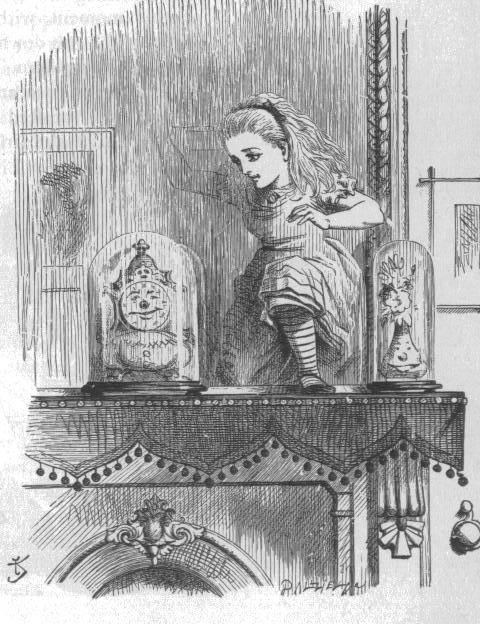
\includegraphics[width=\linewidth]{fig/intro/aliceroom2.jpg}
	\caption{Looking glass room, by John Tenniel.}
\end{marginfigure}

\paragraph*{Constraint Satisfaction Problems.}
Going to the other side, encodings of model-checking problems
as "homomorphism problems" of the form $\textsf{data} \homto^? \textsf{query}$
can be thought of as ``universal problems''---here ``universal'' does not
refer to some form of completeness, but simply to universal quantification.
Notice "eg" that they are anti-monotonic with respect to the data:
for all "structures" $\?A$, $\?A'$ and $\?B$, if $\?A \homto \?B$ and $\?A'$ is a substructure
of $\?A$ then $\?A' \homto \?B$.
Moreover, while problems of the form $\textsf{query} \homto^? \textsf{data}$
can be solved locally---whether a vertex of the data is part of a solution (a "homomorphism") only 
depends on vertices at a bounded distance---, problems of type $\textsf{data} \homto^? \textsf{query}$ cannot.

\begin{marginfigure}[-18em]
	\centering
	\begin{tikzpicture}
		% ---
% 3-clique
% ---
\node[vertex, draw=c0, fill=c0, fill opacity=.4] at (0,0) (k3-0) {};
\node[vertex, above right=1em and 2em of k3-0, draw=c1, fill=c1, fill opacity=.4] (k3-1) {};
\node[vertex, below right=1em and 2em of k3-0, draw=c2, fill=c2, fill opacity=.4] (k3-2) {};

\draw[edge, bend right=15] (k3-0) to (k3-1);
\draw[edge, bend right=15] (k3-0) to (k3-2);
\draw[edge, bend right=15] (k3-1) to (k3-0);
\draw[edge, bend right=15] (k3-1) to (k3-2);
\draw[edge, bend right=15] (k3-2) to (k3-0);
\draw[edge, bend right=15] (k3-2) to (k3-1);
	\end{tikzpicture}
	\caption{
		\AP\label{fig:intro-3-clique}
		The "$3$-clique" $\clique{3}$.
	}
\end{marginfigure}
\begin{marginfigure}[-6em]
	\centering
	\begin{tikzpicture}
		% ---
% Example 3-colouring
% ---
\tikzset{every node/.style={fill opacity=.4}}
\node[vertex, color=c0, fill=c0] at (0,0) (0) {};
\node[vertex, above left=.75em of 0, color=c1, fill=c1] (0al) {};
\node[vertex, above right=.75em of 0, color=c2, fill=c2] (0ar) {};
\node[vertex, below left=2em of 0al, color=c0, fill=c0] (0l) {};
\node[vertex, below right=2em of 0ar, color=c0, fill=c0] (0r) {};
\node[vertex, above left=of 0l, color=c1, fill=c1] (0ll) {};
\node[vertex, above right=of 0r, color=c2, fill=c2] (0rr) {};
\node[vertex, below left=of 0, color=c2, fill=c2] (0bl) {};
\node[vertex, below right=of 0, color=c1, fill=c1] (0br) {};

\node[vertex, below=2em of 0, color=c0, fill=c0] (1) {};
\node[vertex, below left=1em of 1, color=c1, fill=c1] (1bl) {};
\node[vertex, below right=1em of 1, color=c2, fill=c2] (1br) {};
\node[vertex, above left=0em and 1.5em of 1bl, color=c2, fill=c2] (1bll) {};
\node[vertex, above right=0em and 1.5em of 1br, color=c1, fill=c1] (1brr) {};

\node[vertex, below=4em of 1, color=c0, fill=c0] (2) {};
\node[vertex, below left=1.5em and .75em of 1bl, color=c2, fill=c2] (2al) {};
\node[vertex, below right=1.5em and .75em of 1br, color=c1, fill=c1] (2ar) {};
\node[vertex, below left=.5em and 1.5em of 2, color=c1, fill=c1] (2bl) {};
\node[vertex, below right=.5em and 1.5em of 2, color=c2, fill=c2] (2br) {};
\node[vertex, below left=of 2al, color=c0, fill=c0] (2ll) {};
\node[vertex, below right=of 2ar, color=c0, fill=c0] (2rr) {};

\draw[edge] (0) to (0al);
\draw[edge] (0) to (0ar);

\draw[edge] (0al) to (0l);
\draw[edge] (0l) to (0bl);
\draw[edge] (0bl) to (0);
\draw[edge] (0l) to (0ll);

\draw[edge] (0ar) to (0r);
\draw[edge] (0r) to (0br);
\draw[edge] (0br) to (0);
\draw[edge] (0r) to (0rr);

\draw[edge] (0bl) to (1);
\draw[edge] (1) to (1bl);
\draw[edge] (1bl) to (0l);

\draw[edge] (0br) to (1);
\draw[edge] (1) to (1br);
\draw[edge] (1br) to (0r);

\draw[edge] (1bl) to (2al);
\draw[edge] (2al) to (2ll);
\draw[edge] (2) to (2al);
\draw[edge] (2) to (2bl);
\draw[edge] (2bl) to (2al);

\draw[edge] (1br) to (2ar);
\draw[edge] (2ar) to (2rr);
\draw[edge] (2) to (2ar);
\draw[edge] (2) to (2br);
\draw[edge] (2br) to (2ar);

\draw[edge] (1bl) to (1bll);
\draw[edge] (1br) to (1brr);

\draw[edge, bend right=20] (2) to (1bl);
\draw[edge, bend left=20] (2) to (1br);


	\end{tikzpicture}
	\caption{
		\AP\label{fig:dichotomy-ex-3-clique}
		A "$3$-colouring" of some beetle-shaped "graph@@dir".
	}
\end{marginfigure}
\begin{example}[Graph colouring]
	\AP\label{ex:graph-colouring-as-hom}
	Let $k\in\Np$. We let the \AP""$k$-clique"", denoted by $\intro*\clique{k}$,
	to be the "graph@@dir" whose vertices are $\intInt{1,k}$,
	and with an edge from $i$ to $j$ (with $i,j \in \intInt{1,k}$)
	"iff" $i\neq j$, see \Cref{fig:intro-3-clique}.
	The classical graph-theoretical notion of \AP""$k$-colouring""
	of a "graph@@dir" $\?G$ consists of
	a map from vertices of $\?G$ to $\intInt{1,k}$
	"st" no two adjacent vertices are sent on the same colour/number.
	We then say that a "graph@@dir" is \AP""$k$-colourable"" when
	it admits at least one "$k$-colouring".
	In other words, a "$k$-colouring" corresponds precisely to a "homomorphism" from $\?G$
	to $\clique{k}$, where colours correspond to the vertices of the clique,
	see "eg" \Cref{fig:dichotomy-ex-3-clique}.
	Hence, a graph is "$k$-colourable" if, and only if,
	there is a "homomorphism" from $\?G$ to $\clique{k}$.
\end{example}

For instance, "$3$-colourability" is a global property of a graph and cannot be solved
by gluing local solutions, or with greedy algorithms.
In particular, this implies that fixing the query
does not necessarily result in
a drop in the complexity: the \AP ""$3$-colourability problem""---which takes as input a finite "graph@@dir" and asks whether it is "$3$-colourable"---is already "NP"-complete!
The next example shows that, even when the "target structure" is fixed, the "homomorphism problem"
provides a flexible framework to encode problems.

\begin{example}[SAT solving]
	\AP\label{ex:sat-as-hom}
	We consider a 3-SAT instance, namely a finite conjunction of
	disjunctions of three literals, say
	\[
		\phi \defeq \bigwedge_{i=1}^n \ell_{i,1} \lor \ell_{i,2} \lor \ell_{i,3},
	\]
	where each $\ell_{i,j}$ is either a variable, or the negation of a variable.
	We assume "wlog" that in each clause, positive variables appear before negative ones:
	this of course can be achieved by a simple syntactical rewriting of each clause.%
	\footnote{Meaning "eg" that $x \lor \neg y \lor z$ is not allowed, contrary to
	$x \lor z \lor \neg y$.}
	We let $\?B$ be the structure whose domain has two elements $\{0,1\}$,
	equipped with four ternary relations $\+R_0$ through $\+R_3$, where $\+R_j$ encodes clauses with exactly $j$ negated literals. They are formally defined as
	\begin{align*}
		\+R_0 & \defeq \set{0,1}^3 \smallsetminus \set{\tup{0,0,0}}, &
		\+R_1 & \defeq \set{0,1}^3 \smallsetminus \set{\tup{1,0,0}}, \\
		\+R_2 & \defeq \set{0,1}^3 \smallsetminus \set{\tup{1,1,0}} \qquad\text{ and} &
		\+R_3 & \defeq \set{0,1}^3 \smallsetminus \set{\tup{1,1,1}}.
	\end{align*}
	We then encode $\phi$ into the "relational structure" $\?F_\phi$
	whose domain is the set of variables of $\phi$,
	and for every $i \in \intInt{1,n}$,
	$\+R_j$ ($j\in\intInt{0,3}$) consists of all triplets of variables $\tup{x,y,z}$
	"st" there is a clause of $\phi$ containing variables $x$, $y$ and $z$ (with multiplicity), and exactly $j$ of these variables occur negatively.
	For instance, $\tup{x, y, \neg x} \in \+R_1$, and $\tup{\neg x, \neg y, \neg z} \in \+R_3$.
	A function $f$ from the domain of $\?F_\phi$ to the domain of $\?B$ amounts to picking
	a Boolean valuation of the variables occurring in $\phi$.
	Observe that, by definition of the relations $\+R_j$,
	given a clause $\psi$ containing variables $x,y,z$, 
	$f$ is a "homomorphism" from $\?F_\psi$ to $\?B$ "iff"
	$f$, seen as a valuation, satisfies $\psi$.\footnote{For instance,
	if all variables are positive, then all valuations except the one putting
	all variables to false satisfy the formula. This is why $\+R_0$ is defined
	on $\?B$ as $\set{0,1}^3\smallsetminus \set{\tup{0,0,0}}$.}
	By taking conjunction, the conclusion follows: "homomorphisms" from
	$\?F_\phi$ to $\?B$ exactly correspond to valuations satisfying $\phi$.
	In particular, there is a "homomorphism" from $\?F_\phi$ to $\?B$ "iff"
	$\phi$ is satisfiable.%
	\footnote{Note that this example can be easily generalized to $k$-SAT for any $k\in\Np$.
	However, the "signature" depends on $k$.}
\end{example}

However, contrary to "$3$-colourability" and SAT solving, not all of these problems are NP-hard. For example, $2$-colourability is not only polynomial-time,
but can be solved using a greedy algorithm. This begs the question of understanding what
makes a "relational structure" hard for the "homomorphism problem" when it is used
as the "target structure".
This question is not only motivated by theory: constraint logic programming has emerged in the 1980s
with Prolog II and III; and modern programming languages such as answer-set programming provide an 
efficient way of doing constraint solving.

\begin{figure}
	\centering
	\lstinputlisting[language=myclingo]{fig/intro/sudoku.lp}
	\caption{
		\AP\label{fig:ex-sudoku-asp}
		A Clingo program (answer-set programming) to solve Sudoku grids.
		Written by Enrico Höschler
		\href{https://ddmler.github.io/asp/2018/07/10/answer-set-programming-sudoku-solver.html}{[source]}.
		Try running it on \url{https://potassco.org/clingo/run/}!
	}
\end{figure}

Answer-set programming can be thought of, albeit caricaturally, as a human-readable
SAT-solver. It deals with variables, relations between these variables,
and logical rules between these variables. These rules take the form
\lstinline[language=myclingo]|A :- B|, which can be understood as `if $B$, then $A$'.
The right-hand side is parsed conjunctively while the left-hand side is parsed disjunctively:
\lstinline[language=myclingo]|A, B :- C, D| should be understood as `if $C$ and $D$, then $A$ or $B$'.
\Cref{fig:ex-sudoku-asp} provides
an example of a Clingo program for solving Sudoku grids:
\begin{itemize}
	\item it starts by declaring three types of variables: abscissa $x$, ordinates $y$ and values $n$ (representing a value in the grid), as well as their range;
	\item it introduces a \textsf{sudoku} ternary relation, where $\textsf{sudoku}(x,y,n)$
		represents the fact that entry $(x,y)$ of the grid has value $n$,
		and it says that there should be exactly one value per entry;
	\item it introduces a \textsf{subgrid} relation, saying when two entries
		belong to the same 3$\ast$3-square;
	\item finally, it says that any two values on the same column, row or subgrid
		must be different.%
		\footnote{Recall that the left-hand side of rules is understood disjunctively,
		and hence \lstinline[language=myclingo]|:- A, B| reads as `if $A$ and $B$, then false'.}
\end{itemize}
To solve a specific grid using the program of \Cref{fig:ex-sudoku-asp},
it suffices to add declarations of the form \lstinline[language=myclingo]|sudoku(4,1,5).|,
where \lstinline[language=myclingo]|A.| is a shorthand for \lstinline[language=myclingo]|A :-.|.
This specifies that the cell at position $(4,1)$ has value 5.

Contrary to more classical programming languages, this paradigm does not explain \emph{how} things
should be computed, but \emph{what constraints} the memory/solution should satisfy.
In "homomorphism problems", the "target structure" precisely plays this role of
encoding constraints. For instance, the only constraint for a graph $3$-colouring is that
adjacent vertices must be mapped to distinct colours: this constraint is
reflected in $\clique{3}$ by the fact that the edges of $\clique{3}$ are exactly the pairs
of distinct colours.

The field of \AP""constraint satisfaction problems"" precisely aims at classifying the
structures $\?B$ "wrt" to the complexity of the "homomorphism problem" when the
"target structure" is $\?B$. One of the earliest and most impactful result
of the domain was found by Schaefer \cite{Schaefer1978ComplexitySatisfiability},
who proved that such problems are either in "P" or "NP"-complete when the domain of $\?B$
has two elements---this already captures the example of SAT-solving (\Cref{ex:sat-as-hom}) from earlier.
A decade later, Hell and Ne\v{s}et\v{r}il \cite{HellNesetril1990ComplexityColoring}
proved a similar result for "undirected graphs".
Moreover, in both cases, these dichotomies are effective: given a structure, we can decide if
its "homomorphism problem" is in "P" or is "NP"-complete.
These results, together with the importance of \emph{constraint satisfaction} in computer science
led Feder and Vardi at the end of the 1990s
to state their celebrated \emph{dichotomy conjecture}: ``for any "finite structure" $\?B$,
the "homomorphism problem" with "target structure" $\?B$ is either "P"
or "NP"-complete'' \cite{FederVardi1998ComputationalStructure}.
Despite receiving lots of attention, the conjecture remained wide open for two decades, until
Bulatov \cite{Bulatov2017DichotomyCSPs} and Zhuk \cite{Zhuk2020CSPDichotomy} independently
showed the conjecture to be true.%
\footnote{Both papers have in fact been first published in 2017 in the same conference:
\cite{Zhuk2020CSPDichotomy} refers to Zhuk's later journal version.}

However not all problems in "P" are complete for this class: some are even simpler and are complete
for "NL" or "L", or even "FOfin"---i.e. when it is a "first-order definable" class of "finite structures".
One result that will be of major importance in this thesis is a dichotomy
theorem by Larose and Tesson separating "structures" in "FOfin" from those that are "L"-hard
\cite{LaroseTesson2009UniversalAlgebraCSP}.

\begin{known}
	The field of constraint satisfaction problems classifies "target structures"
	depending on the complexity of their "homomorphism problem".
\end{known}

\subsection{Automatic Structures: The Dream Is Not Over Yet}

The second part of this thesis is dedicated to pushing these results to their limit.
The "structures" handled by the "homomorphism problem", like most
problems in computer science, are usually assumed to be "finite@@struct".
We discuss in this section the generalization of the problem to
infinite structures. This motivated by two facts: not only infinite structures
naturally arise as from computational models---the runs of a machine
usually form an infinite "structure"---, they can also model `mathematical universes'.

Von Neumann would have said ``It's all over''%
\footnote{This quote is mentioned as historically accurate by
\cite{2009Logicomix}, however this claim seems undocumented \cite{Mancosu2011Logicomix}.}
after hearing Gödel expose his infamous "incompleteness theorem" in 1930:
any \emph{effective} (recursively enumerable)
consistent theory that is expressive enough to express the arithmetic
is incomplete---"ie" it contains statements that are neither valid (true in all models),
nor unsatisfiable (false is all models).
In other words, there is no reasonable set of axioms
to capture all mathematics: some statements must necessarily fall outside
the scope of the theory.
\begin{marginfigure}[-55em]
	\centering
	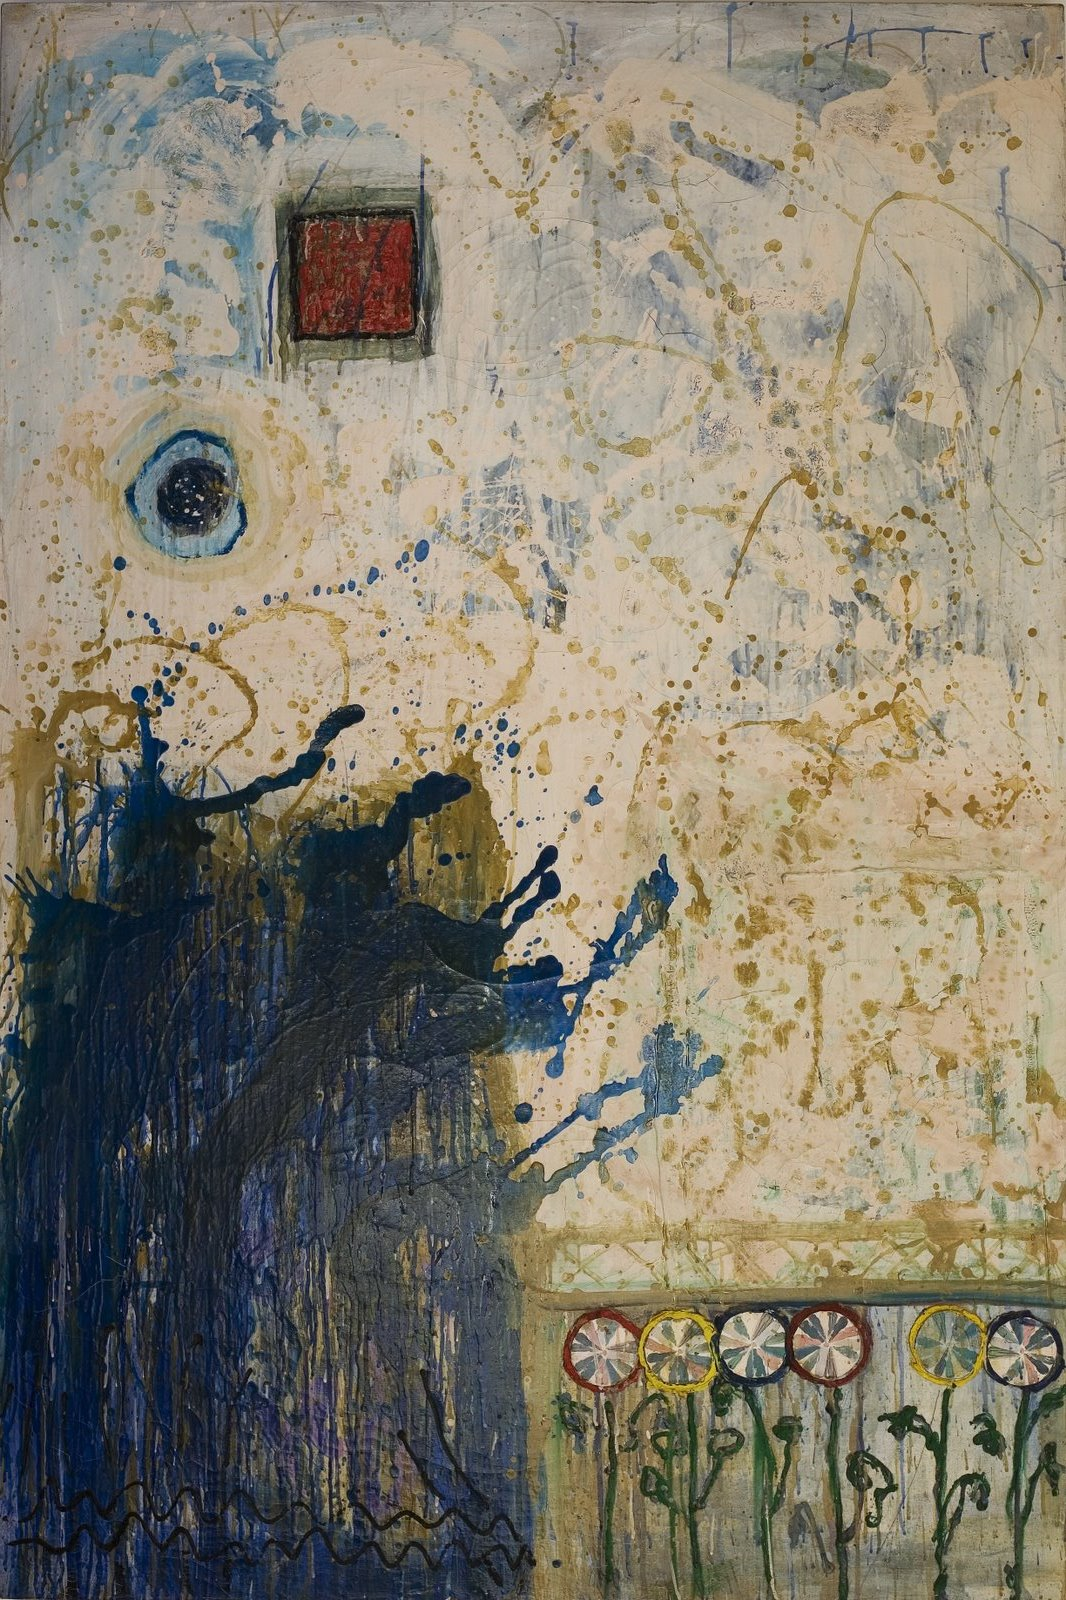
\includegraphics[width=\linewidth]{fig/Flowers_for_Algernon.jpg}
	\caption{\emph{\href{https://commons.wikimedia.org/wiki/File:Flowers_for_Algernon.jpg}{Flowers for Algernon}}, Marshall P Baron.
	Licensed under "CC BY SA 4.0".}
\end{marginfigure}
\marginnote{\blockquote[Daniel Keyes, \emph{Flowers for Algernon}]{Another case of men devoting their lives to studying more and
more about less and less.}}

Completeness is perhaps best understood as follows:
if a theory (a set of axioms) is consistent---"ie" it has at least one model---and complete, 
then pick any of its models. A statement is then valid in the theory if and only
if it is true in this model. Dually, if you are given a theory for which
there exists a model with this property (a statement is valid in the theory "iff" it
is true in the model), then the theory is complete.
In essence, not only does Gödel's result put a dent in Hilbert's dream
(``Wir müssen wissen. Wir werden wissen.''%
\footnote{``We must know. We will know.''}) of building solid foundations for mathematics:
in fact, it shatters the Platonistic idea of an unequivocal and universal mathematical world, or 
at the very least of one that can be captured by axioms.

Ironically, what makes "Gödel's incompleteness theorem" a proper
abomination for computer scientists is probably another theorem of Gödel,
known as "Gödel's completeness theorem" and that he proved
only a year earlier in his Ph.D. dissertation: 
first-order logic admits a complete proof system. Or, said differently,
what is valid---that is, true on every model satisfying the axioms---is exactly what
can be proven. 
Hence, the Gödel of 1929 could have dreamt of a complete theory for mathematics.
If a such theory existed, to determine if a statement $\phi$ was valid, it would suffice
to enumerate in parallel all possible proofs of $\phi$ and of $\neg \phi$. By completeness, this 
procedure would always stop, and either conclude that $\phi$ is valid, or that
$\neg \phi$ is valid.%
\footnote{Formally: any recursively enumerable complete first-order theory is decidable.}
Are there cardinals strictly between $\aleph_0$ and the continuum?
Start Turing's nifty device---invented in 1936---, and you would (eventually) get an answer! In this strange world, automatic theorem proving would be a reality,
and this thesis would probably look very different.

Sadly for the Gödel of 1929, the Gödel of 1930 came, and so… ``It's all over''!
Since then, theories---such has
"Zermelo–Fraenkel set theory plus the axiom of choice"---have been developed, and while not being complete, they 
manage to capture most of the parts of mathematics we are interested in.%
\footnote{For the sake of sanity, we assume
throughout this introduction that the pronoun `we' excludes set theorists.}
\begin{marginfigure}
	\centering
	\[
	\contraction{}{\tau\,}{{\vee} {\neg} {\in}}{\!\square}
	\contraction[2ex]{}{\tau\!}{{\vee} {\neg} {\in} \square A' {\in}}{\square}
	\tau {\vee} {\neg} {\in} \square A' {\in} \square A''
	\]
	\caption{\AP\label{fig:intro-bourbaki}
	The "first-order sentence" $\exists x.\, (x \not\in A') \lor (x \in A'')$
	as written by Bourbaki in \cite[\S~1]{Bourbaki2006Logique}.
	}
\end{marginfigure}
\begin{marginfigure}
	\centering
	\[
		\Fanqn{x}\Fconditional{\Fcontent x \in A''}{\Fcontent x \in A'}
	\]
	\caption{\AP\label{fig:intro-frege}
		The "first-order sentence" of \Cref{fig:intro-bourbaki}
		written using Frege's notations (1879).
	}
\end{marginfigure}
Yet, after half a century of efforts to build solid foundations,
the incompleteness of this consolation prize is actually frustrating,
and mathematicians still often resort to denial.
\begin{displayquote}[Jean Dieudonné {\cite{Dieudonne1970Bourbaki}}]
	``On foundations we believe in the reality of mathematics, but of course when philosophers attack us with their paradoxes we rush to hide behind formalism and say: ``Mathematics is just a combination of meaningless symbols,'' and then we bring out Chapters 1 and 2 on set theory. Finally we are left in peace to go back to our mathematics and do it as we have always done, with the feeling each mathematician has that he is working with something real.
	This sensation is probably an illusion, but is very convenient. That is Bourbaki's attitude towards foundations.''
\end{displayquote}
For the reader intrigued by what could possibly frighten philosophers in Bourbaki's first volume,
we refer them to the formula of \Cref{fig:intro-bourbaki}---interestingly, this is not the most 
frightening way to write formulas, see \Cref{fig:intro-frege}!

However, not all hope is lost: while the Platonistic mathematical world might
not be understood, some of it restrictions might be axiomatized.
In 1929, Presburger proved that a natural set of axioms for doing
arithmetic with only addition is also both complete and decidable---the formulas
that are valid in this theory exactly correspond to the sentences that are true on $\tup{\N,+}$.
Around the same time, Tarski formalized Euclide's geometry as a first-order theory, and proved
that is was complete and decidable, see \cite{TarskiGivant1999Geometry}.

Hence, logic is not completely useless at capturing complex infinite structures!
Interestingly, generalizing the idea behind the decidability of Presburger's arithmetic,
mathematicians and computer scientists kept 
rediscovering the notion of "automatic structures" during the second half
of the XXth century.%
\footnote{It should be noted that while the most common way of proving
the decidability of Presburger's arithmetic today is by using
automata, this is not Presburger's original proof, who relies on quantifier elimination.}
This notion captures the idea on why $\tup{\N,+}$ can be simply axiomatized:
in this sense "automatic structures" salvage the shards of mathematicians' shattered dreams.
Given an "automatic structure" and a "first-order sentence",
we can decide whether it holds on this "structure". These structures can be infinite,
but are, by definition, describable by finite-state automata---which is what
makes decidability possible.

\begin{known}
	The first-order theory of every "automatic structure" is decidable.
\end{known}

Unsurprisingly, the foremost example of an "automatic structure" is $\tup{\N, +}$.%
\footnote{See \Cref{ex:presburger}.}
On the other hand, it should be noted that Peano's arithmetic, namely natural number with
addition and multiplication $\tup{\N,+,\cdot}$ is not "automatic@@struct",
as it is already undecidable.
While "automatic structures" cannot express ``mathematical universes'' serving as
foundations for a universal mathematical theory, they are surprisingly adequate to
express infinite "structures" arising from computational models.
For instance, the graph of runs of a finite-state automaton is "automatic@@struct",
since the unfolding of any finite graph is "automatic@@struct".
Even more generally, the "configuration graph" of any "Turing machine" is "automatic@@struct"...%
\footnote{See \Cref{ex:turing-machine-are-automatic}.}

Hence, in \Cref{ch:dichotomy-theorem}, we naturally study the "homomorphism problem" when the "source structure"
is allowed to be any "automatic structure". Surprisingly, very little was known about this problem:
the only known result by Köcher states that whether an "automatic graph" is "2-colourable" is undecidable \cite{Kocher2014AutomatischenGraphen}.
Said otherwise, it is undecidable whether an "automatic graph" admits
a "homomorphism" to the "$2$-clique".
This led us to conjecture that actually most "homomorphism problems" on "automatic structures"
should be undecidable, since $\clique{2}$ is actually somewhat ``simple''.

While the "homomorphism problem" seems quite natural at first glance, a "homomorphism" $f$
from an "automatic structure" $\?A$ to a "finite one@finite structure" $\?B$ does not live
in the same world as $\?A$ and $\?B$, in the sense that it might not be finitely presentable---its domain is infinite and so, \emph{a priori} require infinite information to be described.
We introduce the notion of "regular homomorphisms", that corresponds to "homomorphisms" that
are finitely presentable in the same fashion as "automatic structures", and show that
this notion differs from the notion of "homomorphism",
see \Cref{fig:tree-not-2reg-colour,ex:tree-not-2-reg-colourable}.

\begin{marginfigure}
	\centering
	\begin{tikzpicture}
		% ---
% 3-transitive tournament
% ---
\node[vertex, draw=c3, fill=c3, fill opacity=.4] at (0,0) (t3-3) {};
\node[vertex, above=of t3-3, draw=c2, fill=c2, fill opacity=.4] (t3-2) {};
\node[vertex, above=of t3-2, draw=c1, fill=c1, fill opacity=.4] (t3-1) {};
\node[vertex, above=of t3-1, draw=c0, fill=c0, fill opacity=.4] (t3-0) {};

\draw[edge] (t3-0) to (t3-1);
\draw[edge] (t3-1) to (t3-2);
\draw[edge] (t3-2) to (t3-3);
\draw[edge] (t3-0) to[bend left=60] (t3-2);
\draw[edge] (t3-1) to[bend left=60] (t3-3);
\draw[edge] (t3-0) to[bend right=60] (t3-3);
	\end{tikzpicture}
	\caption{
		\AP\label{fig:3-transitive-tournament}
		The "$3$-transitive tournament" $\transitiveTournament{3}$.
	}
\end{marginfigure}
Our first contribution is to show that whether a graph admits a "regular $2$-colouring" is undecidable. We then notice that a particular type of
"homomorphism problem" is decidable: for instance, if the "target structure"
is a "transitive tournament". This is best understood on an example: consider the "$3$-transitive 
tournament" depicted in \Cref{fig:3-transitive-tournament}.
A "homomorphism" $f$ from a graph $\?G$ to $\transitiveTournament{3}$ amounts to a function
from the set of vertices of $\?G$ to $\intInt{0,3}$ "st"
for any vertices $u$ and $v$, if there is an edge from $u$ to $v$, then
$f(u) < f(v)$. It is clear that the existence of such a mapping is in fact equivalent 
to asking that there is no path of length $4$ in $\?G$.
In turn, this property can be expressed by a "first-order formula", and is hence decidable
on "automatic graphs".
More generally, this property can be extended to any "target structure" $\?B$ with the property
that the class of (finite or infinite) "structures" $\?A$ that admit a "homomorphism" to $\?B$
is "first-order definable".
Luckily for us, this class has been well-studied, and is known as the class of "structures"
with "finite duality" \cite{Atserias2008DigraphColoring}. In particular, let us cite the result of Larose and Tesson
who proved that any "homomorphism problem" whose "target structure" does not have "finite duality"
must be "L"-hard \cite{LaroseTesson2009UniversalAlgebraCSP}.

The "homomorphism problem" on "automatic structures" 
is undecidable when the "target structure" is a finite "clique".
Yet, it becomes decidable when the target is a finite "transitive tournament".
This contrast leads to conjecture that "finite duality" represents the frontier of decidability for "automatic structures". In \Cref{ch:dichotomy-theorem}, we manage to prove this result, and extend it to "regular homomorphisms".

\begin{contribution}
	We provide a dichotomy theorem for "automatic structures":
	for any "finite structure" $\?B$, the "homomorphism problems" with "target structure" $\?B$
	is either in "NL" or is undecidable. The same holds for "regular homomorphisms".
	Moreover, in both cases, these two problems are decidable precisely when $\?B$ has "finite duality".
\end{contribution}

Part of the proof, namely the `undecidability' part, are proven
by generalizing Larose and Tesson's reduction, although proving that the
`base problem' of the reduction is undecidable is non-trivial.
For proving the decidability of "regular homomorphisms" when $\?B$ has finite duality,
we provide two alternative proofs: a logical-one---which is quite abstract but somewhat short---and
a graph-theoretical one---the algorithm is much more concrete, but the proof of correctness is 
quite long. This last proof actually provides new hindsights on an existing algorithm from the literature, called "hyperedge consistency algorithm@@finite".

Since the "configuration graph" of any "Turing machine" is an "automatic graph",
it follows that this dichotomy theorem\footnote{See \Cref{thm:dichotomy-theorem-automatic-structures} for a formal statement.} can be understood
as a variation on "Rice's theorem", that states that any non-trivial
semantical property of a Turing machine is undecidable.
Our dichotomy theorem hence implies the following result.

\begin{contribution}
	Any non-trivial---"ie" "non-first-order definable"---property on the "configuration graph"
	of a "Turing machine" is undecidable, provided that this property can be expressed
	as a "homomorphism problem".
\end{contribution}

One of our motivations for studying this problem was actually originating
in the "$\AUT$/$\REC$-separability problem", which takes as input two "automatic relations"---namely are binary relations over finite words described by "synchronous automata"---and asks if they can be
"separated@@rel" by a "recognizable relation", "ie" a finite union $\bigcup_i K_i \times L_i$
of Cartesian products of "regular languages". 
We prove this problem to be equivalent to the one taking an "automatic graph" and asks
if it has a finite "regular colouring", which amounts to testing
if there exists some $k\in\Np$ for which the graph admits a "regular homomorphism" to
$\clique{k}$. We still don't know whether this problem is decidable, 
even if the results of \Cref{ch:dichotomy-theorem} hints at its undecidability.
Our undecidability result for "regular homomorphisms"
actually yield, when translated back to the vocabulary of separability,
that it is undecidable whether two "automatic relations" are "separable@@rel"
by a "recognizable relation" that can be written as
a finite union of $k$ Cartesian products, whenever $k \geq 2$ is \emph{fixed}.

\subsection{Language-Theoretic Properties of Presentations of Automatic Structures}

When dealing with "regular languages",
separability problems are quite common:
given a class $\+C$ of "regular languages", understanding
when two "regular languages" can be separated by a language from $\+C$
usually requires a much deeper understanding of the class $\+C$ than
solving the membership problem for $\+C$. In some sense, solving
this latter problem only requires a qualitative understanding of $\+C$,
while the separability problem requires quantitative knowledge on the class. 
A remarkably efficient tool
to prove them decidable is algebraic language theory:
this theory associates to every language a canonical algebra, called "syntactic monoid",
with the property that it is finite if, and only if, the language is "regular@@lang".
Moreover, the language-theoretic and logical properties of the language can be
translated to algebraic properties of this "monoid": more formally, there is a natural
bijection between classes of finite "monoids" and classes of
"regular languages" under mild closure assumptions.

\begin{known}
	Algebraic properties of finite "monoids" correspond to
	language-theoretic and logical properties of "regular languages".
\end{known}

In \Cref{ch:algebra}, motivated by the "$\AUT$/$\REC$-separability problem",
we introduce an algebraic theory for "automatic relations": these algebras are called
"synchronous algebras".
We prove that each finite-word relation%
\footnote{A finite-word relation is simply a subset
$\+R \subseteq \Sigma^* \times \Sigma^*$ for some finite alphabet $\Sigma$.}
admits a "syntactic synchronous algebra",
and that this algebra is finite if, and only if, the relation is "automatic@@rel".

We then prove that classes formed of "these algebras@synchronous algebras" 
are in bijection with the classes of "automatic relations", under some mild closure
assumptions. 

\begin{contribution}
	We extend algebraic language theory to handle relations of finite words
	rather than only languages of finite words.
\end{contribution}

Furthermore, we show that this algebraic theory is relevant, in the following sense.
A "synchronous automaton" encodes a pair (from a binary relation) as
a finite word. This encoding is injective, but not
surjective: not all finite words correspond to encodings of pairs.
Hence, the semantics of a "synchronous automaton" can be precisely seen
as the semantics of a classical automaton, together with the promise that it will be only
fed inputs that corresponds to valid encodings. In other words,
the behaviour of such an automaton on words that do not correspond to a valid encoding
plays no role whatsoever in its semantics, see \Cref{fig:intro-projection}.

\begin{marginfigure}
	\centering
	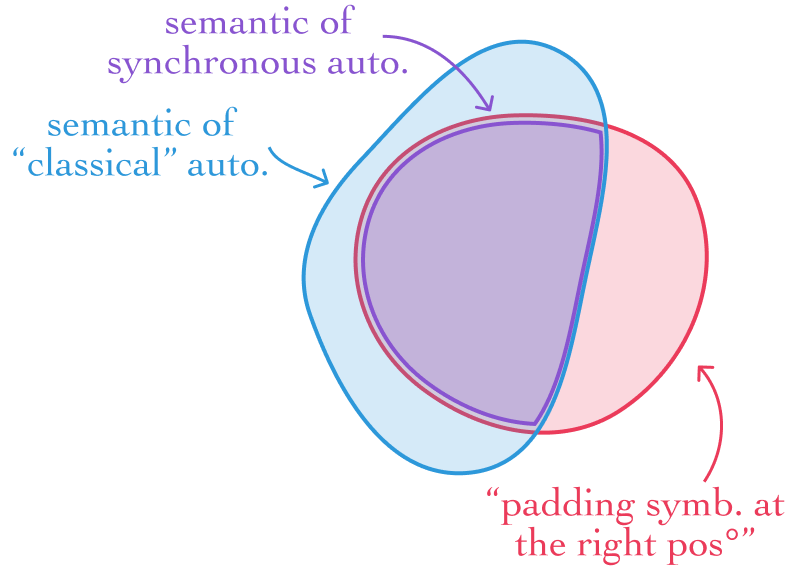
\includegraphics[width=\linewidth]{fig/intro/projection.png}
	\caption{\AP\label{fig:intro-projection}
		Semantics of a "synchronous automaton".
	}
\end{marginfigure}
This approach is ubiquitous in mathematics, and especially in logics:
for instance, first-order logic over "finite structures" is precisely
defined as first-order logic over all "structures", restricted to "finite structures"!
While being natural and ubiquitous, this construction fails to preserve most properties of the logics:
for instance, first-order logic over all "structures" admits a complete proof system,
but does not when restricted to "finite structures". The model-checking problem
is "coRE"-complete over all "structures", but goes to
"RE"-complete---an incomparable complexity class---for "finite structures".
Proving a meta-theorem on such a restriction that explains how some property
behaves in the restricted universe simply by knowing how it behaves on
the larger universe is hence somewhat unexpected but very welcomed!

\begin{contribution}
	We prove that, for any class of "regular languages" satisfying mild closure
	properties, assuming we can decide if a language belongs to this class,
	then we can decide if an "automatic relation" can be written as the restriction
	of a "regular language" in this class to the set of all valid encodings
	of pairs of words.
\end{contribution}

Let us point out that actually, to arrive at this result the notion
of "synchronous algebras" is somewhat intricate. While a more naive definition
exists and makes sense, we show that such a result cannot be proven using this
simpler notion.

This algebraic theory could provide an interesting framework to
study the "$\AUT$/$\REC$-separability problem".
While the class of "recognizable relations" has some desirable
closure properties we need, it lacks others:
unfortunately, it implies that proving the decidability of
the "$\AUT$/$\REC$-separability problem" "via" this framework would
be highly non-trivial.

\begin{openproblemintro}
	Can we decide, given two "automatic relations", if they are "separable@@rel"
	by a "recognizable relation"?
\end{openproblemintro}

In summary, this thesis explores two fundamental perspectives on "homomorphism problems":
the first extends the theory of "conjunctive queries" in database theory by adding regular path
predicates, to capture natural query languages for human-centered graph-shaped data.
It focuses on the problem of query minimization, both in terms of
its total number of atoms, or its tree-width, which is a relevant parameter to
capture the complexity of its evaluation.
The second part focuses on the complexity of problems related to constraint satisfaction
over automatic structures. We show that most \emph{structural} problems, probing the shape of the 
infinite object at hand, are undecidable. In contrast, \emph{language-theoretic} 
problems, dealing with how these infinite structures are represented---or rather how easy it
is to represent them---, remain decidable.